
\chapter{Introduction}

This paper will begin by 

\section{Overview of CDCS}

CDCS is the University's official tool for 

\label{fig:cdcs-index}

\subsection{``Better CDCS''}

%%%

\section{Overview of Skedge}

Skedge is a website on which I started rapid development on December 9th 2013, and have been developing it on and off since.

Bookmarks

Students, parents, department coordinators, and faculty can all benefit from such tool improvements.

user accounts are lightweight, no login, cookie (browser) based

\ref{fig:sk-index}


\begin{figure}[ht]
    \centering
        \begin{subfigure}[h]{14cm}
            \centering
            \fbox{
                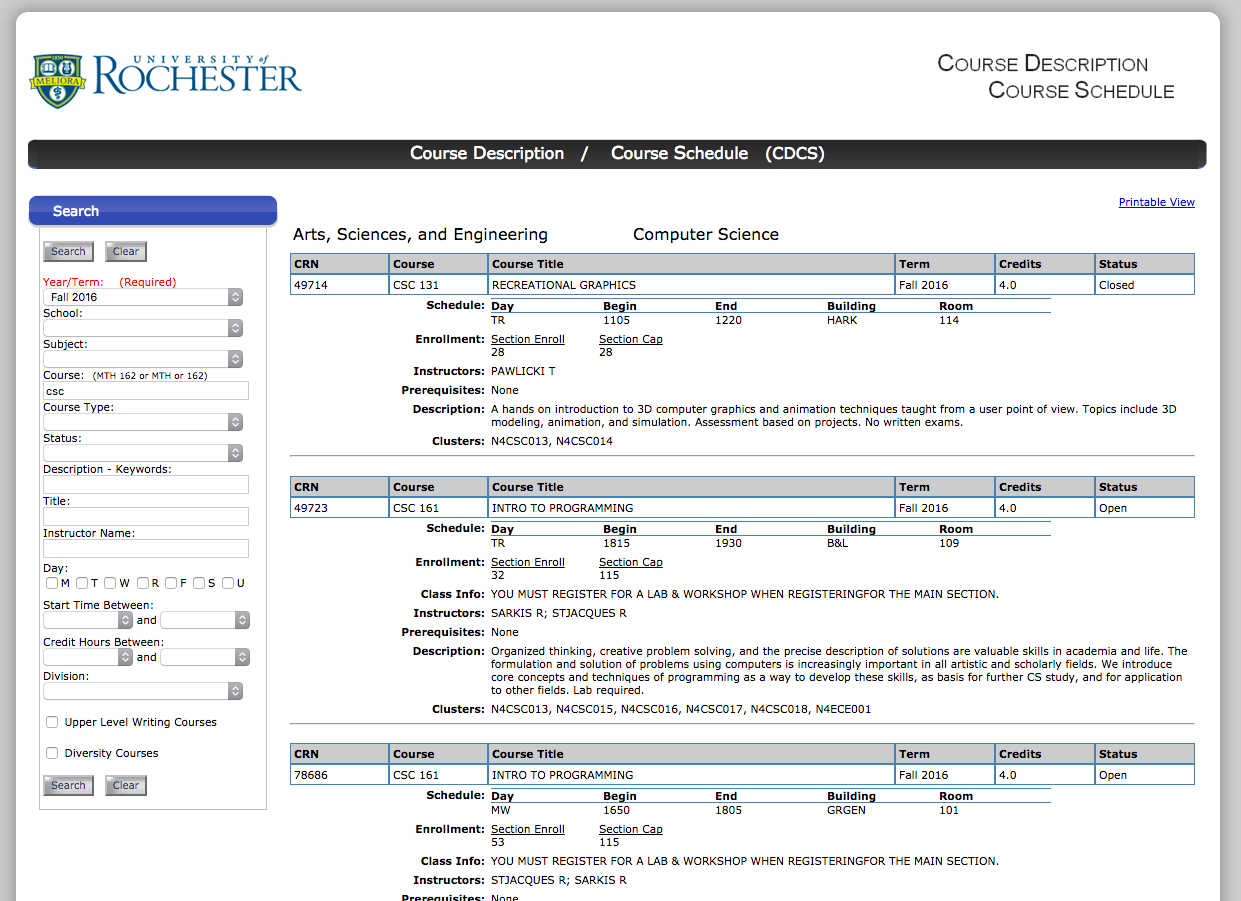
\includegraphics[width=1.00\textwidth]{images/cdcs/index}
            }
            \caption{CDCS, with the search query {\tt csc}}
            \label{fig:cdcs-index}
        \end{subfigure}\\
        \vspace{10pt}\\
        \begin{subfigure}[h]{14cm}
            \centering
            \fbox{
                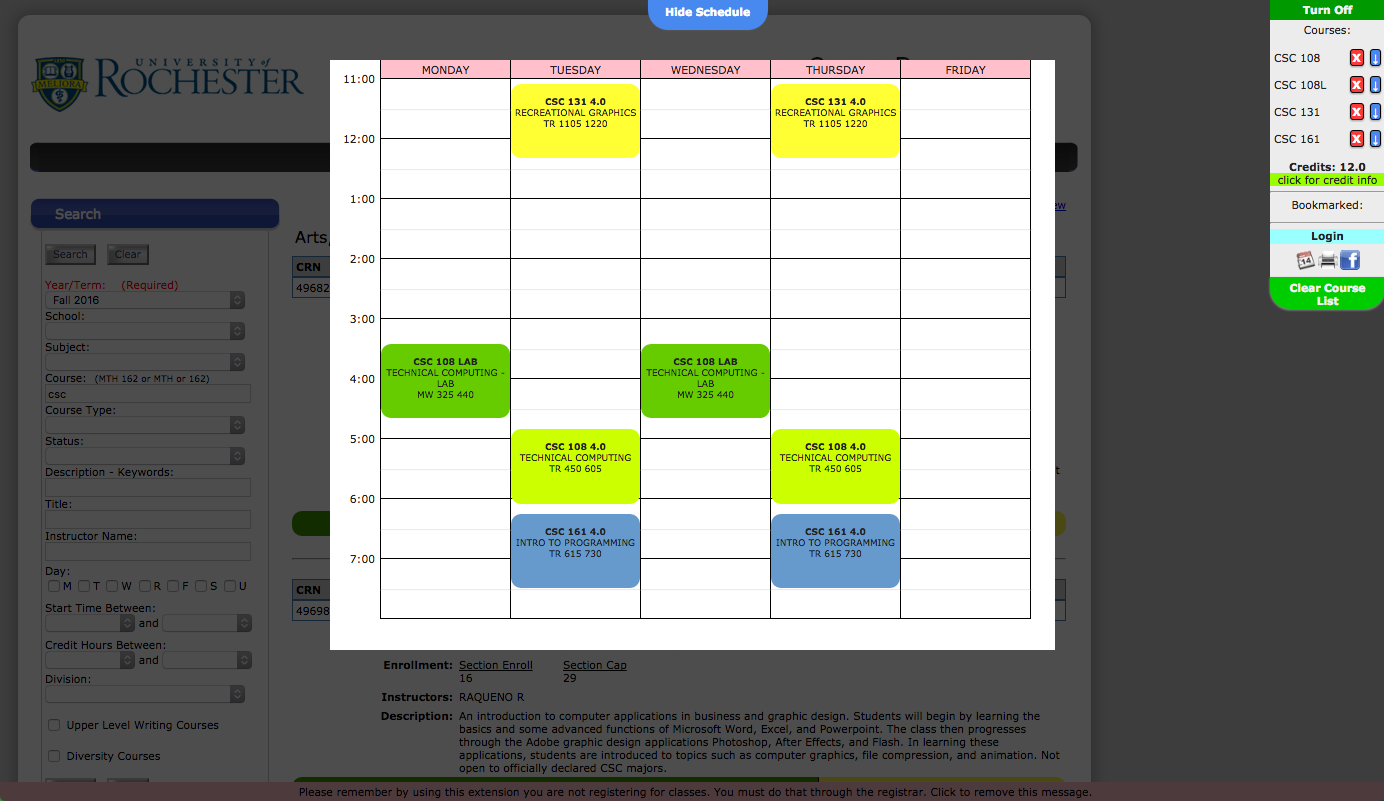
\includegraphics[width=1.00\textwidth]{images/cdcs/better}
            }
            \caption{Better CDCS, a separate browser extension that embeds buttons into the CDCS course results interface, allowing users to add courses to a locally-stored schedule}
            \label{fig:cdcs-better}
        \end{subfigure}
    \caption{CDCS and Better CDCS in their current states}
\end{figure}

\begin{figure}[ht]
    \centering
    \fbox{
        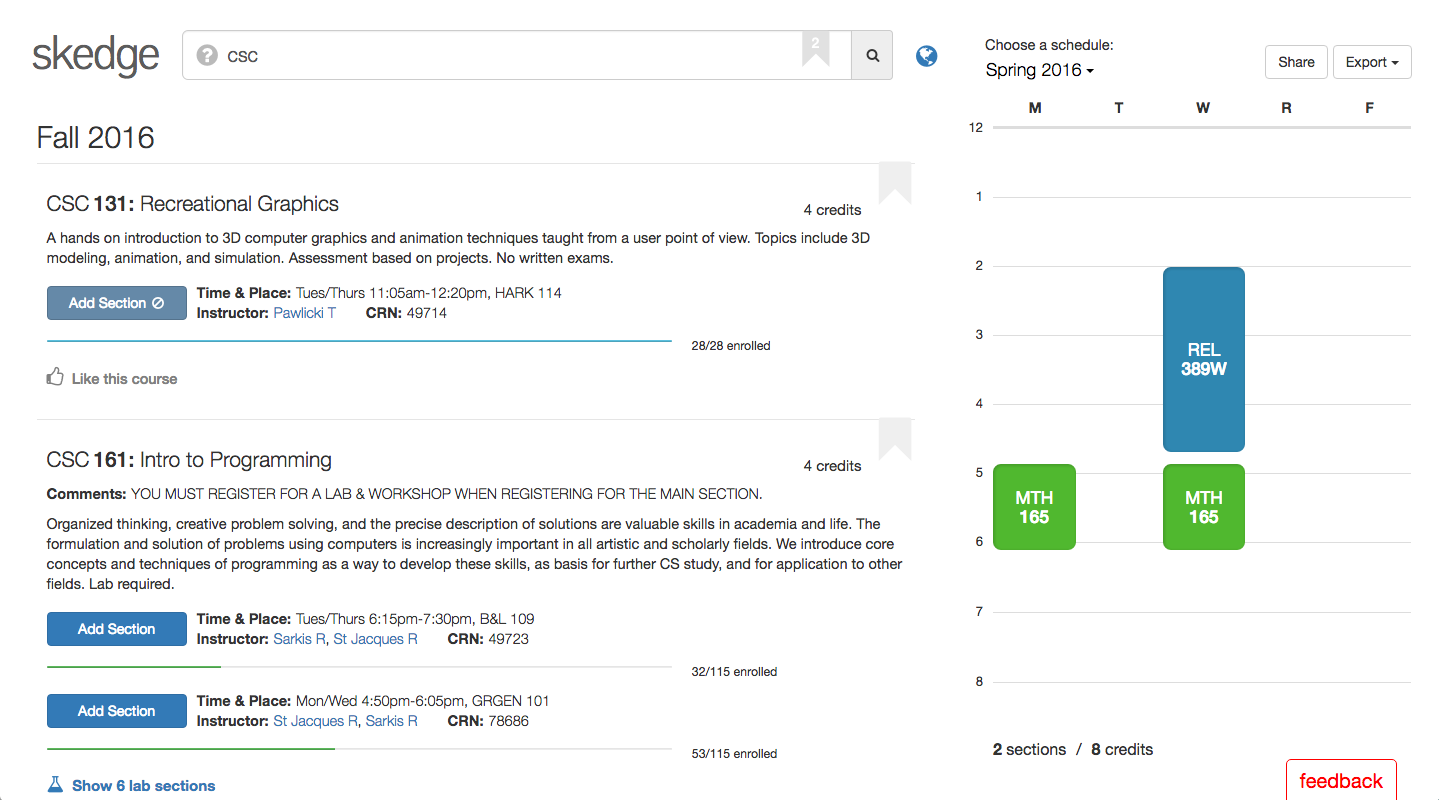
\includegraphics[width=1.00\textwidth]{images/skedge/index}
    }
    \caption[Skedge with the search query {\tt csc}]{Skedge with the search query {\tt csc} and the user's current schedule on the right}
    \label{fig:sk-index}
\end{figure}